\input ../SlidePreamble
\input ../preamble

\begin{document}

{\Huge
  \centerline{\bf TTIC 31230,  Fundamentals of Deep Learning}
  \vfill
  \centerline{David McAllester, Autumn 2022}
  \vfill
  \centerline{\bf History of Deep Learning Part Two}

\vfill
\vfill

\slide{Wav2vec 2.0, June 2020, Facebook}

\vfill
Trained on 53k hours of unlabeled audio (no text) they convert speech to a sequence of discrete quantized vectors they call ``pseudo-text units''.

\vfill
By training on only one hour of human-transcribed audio, and using the Wav2vec transcription into pseudo-text, the outperform the previous state of the
art in word error rate for 100 hours of human-transcribed text.


\slide{GLSM, February 2021, Facebook}

Generative Spoken Language Model (GLSM)

\vfill
They then train a generative model of the sequences of pseudo-text units learned from unlabeled audio.


\vfill
This model can continue speech from a speech prompt in much the same way that GPT-3 continues text from a text prompt.

\vfill
Semantic and grammatical structure in a ``unit language model'' is recovered
from speech alone.

\slide{Codex, July 2021, OpenAI}

This is a language model trained on code, including comments, from public repositories.

\vfill
Starting from an English prompt Codex continues with code --- a form of automatic programming.

\vfill
There is a published version (58 authors) and a production version that powers {\bf GitHub Copilot}.

\vfill
Copilot may supplant Stack Overflow for finding out how to do x in language y.

\slide{CLIP, January 2021, OpenAI}

CLIP: Contrastive Language-Image Pre-training.

\vfill
Trained on images and associated text (such as image captions or hypertext links to images) CLIP computes embeddings of text and embeddings of images
(``co-embeddings'') trained to capture the mutual information between the two.

\vfill
This is done with contrastive learning.

\slide{CLIP, January 2021, OpenAI}

The model computes a probability of text given the co-embedding of the image.

\vfill
It is then used for zero-shot image classification on various datasets.

\vfill
One can classify an image by comparing the probabilities that the model assigns to ``prompts''.  There is a prompt for each class.

\slide{Zero-Shot Image Classification}

\centerline{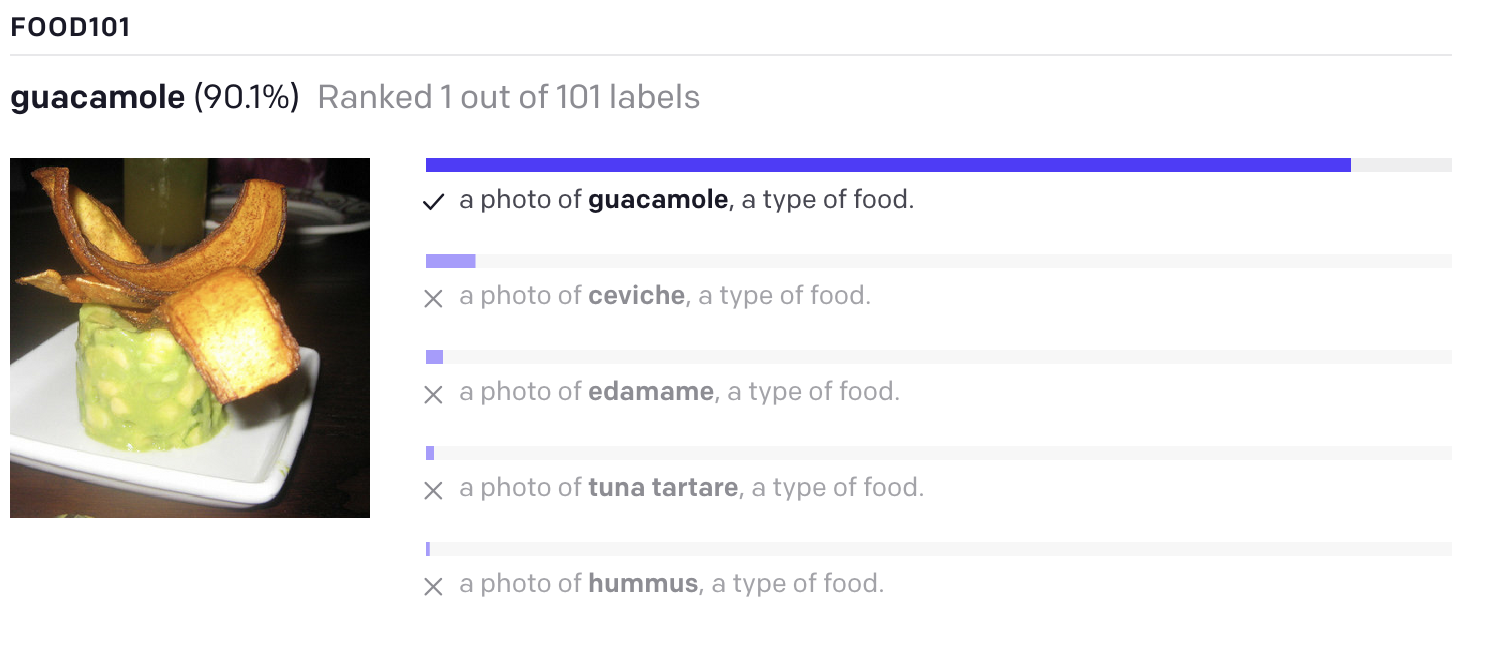
\includegraphics[width = 7in]{\images/CLIP0}}

\slide{Zero-Shot Image Classification}

\centerline{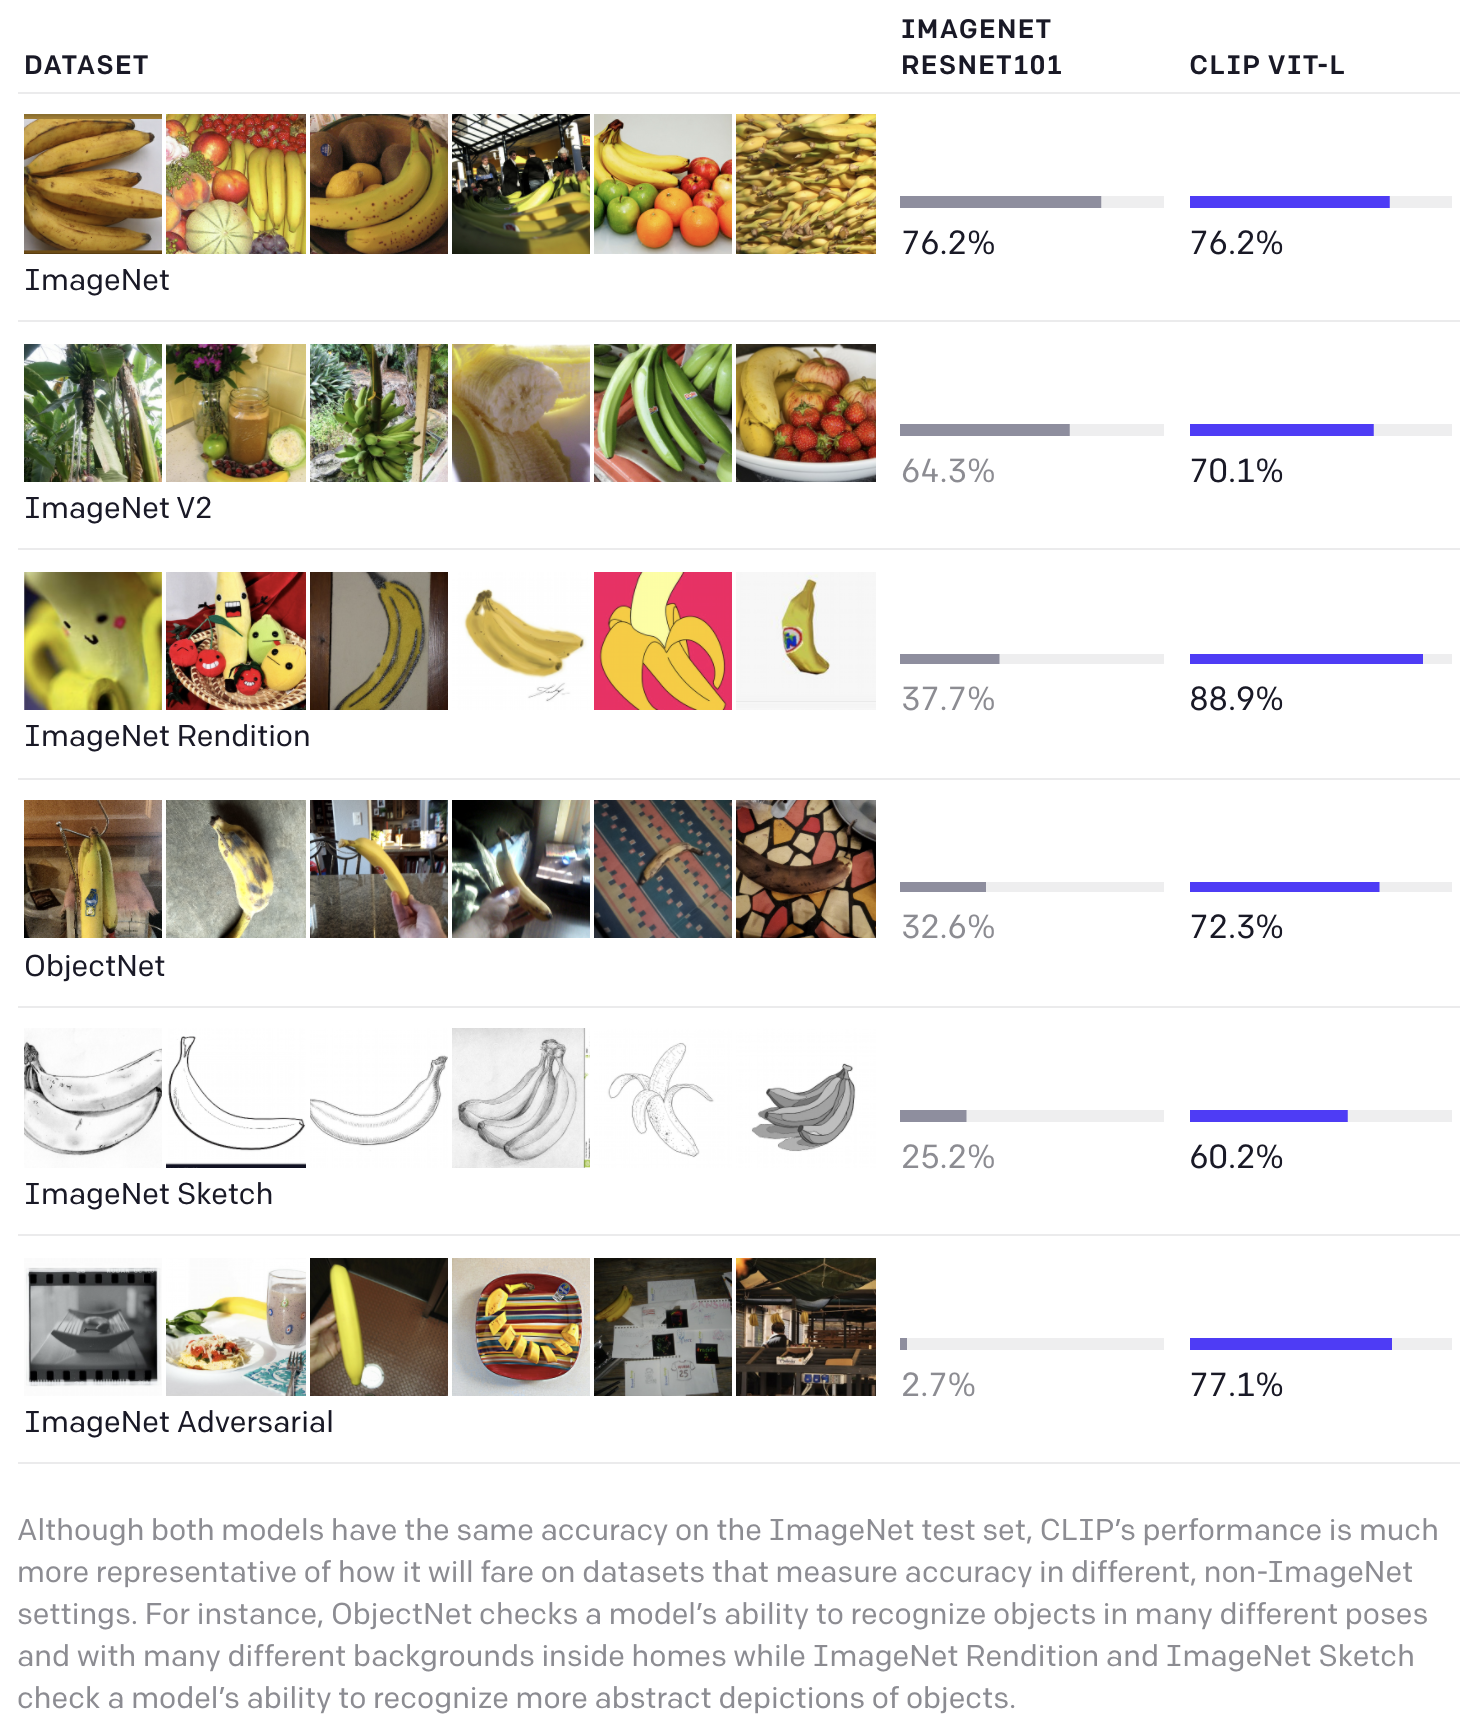
\includegraphics[height= 5in]{\images/CLIP1}}

\slidetwo{DALL$\cdot$E, January 2021, OpenAI}{DALL$\cdot$E-2, April 2022}


The name DALL$\cdot$E is simply some kind of homage to the painter Dali and the Disney character WALL$\cdot$E.

\vfill
Both versions of DALL$\cdot$E uses CLIP's co-embeddings of images and text.

\vfill
Given text, DALL$\cdot$E generates an image.

\slide{DALL$\cdot$E-1 Zero-Shot Image Rendering from Language}

\centerline{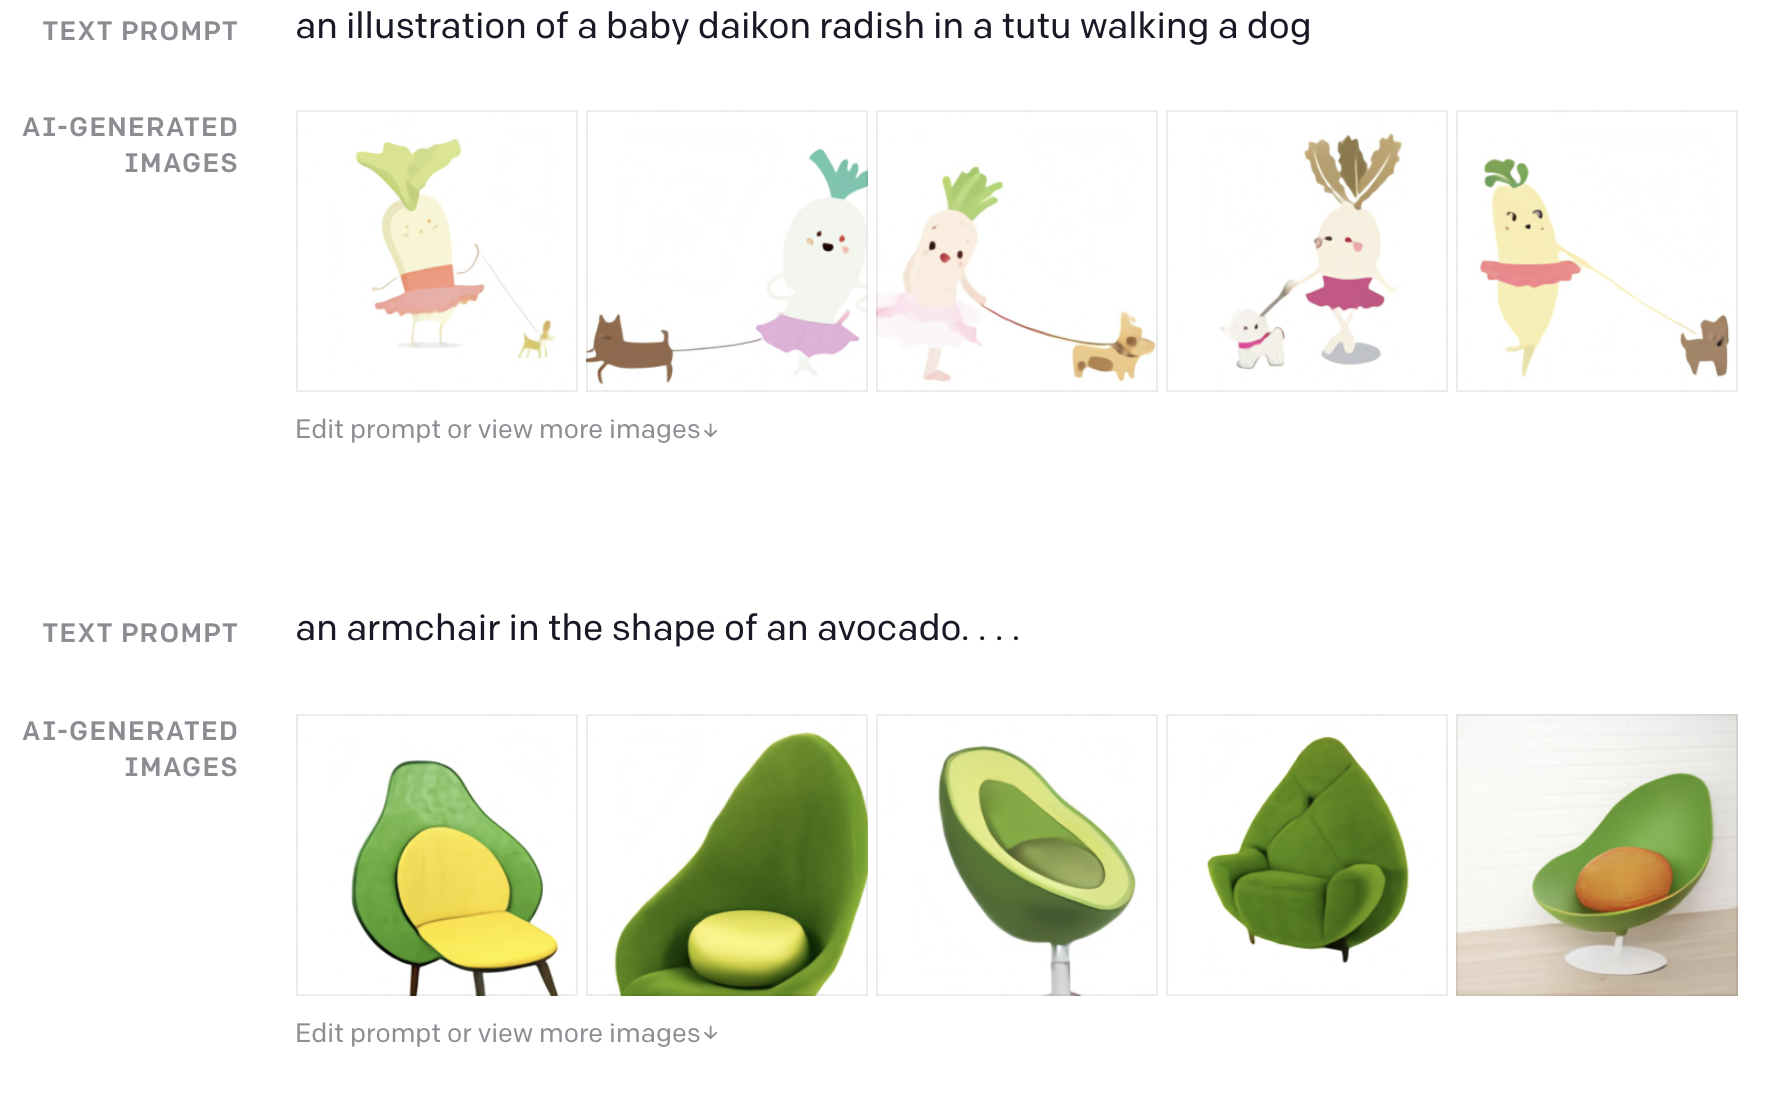
\includegraphics[height= 5in]{\images/DALLE1}}

\slide{DALL$\cdot$E-2}

\centerline{\includegraphics[height= 5in]{\images/DALLE2}}

\slide{Diffusion Models}

DALL$\cdot$E-2 uses diffusion models.  Although originally defined in 2015, they have become very prominent in the last year.

\slide{Chain of Thought Prompting, January 2022}

Give examples of ``chains of thought'' for few shot learning of reasoning steps.

\slide{Naive Prompting}

\centerline{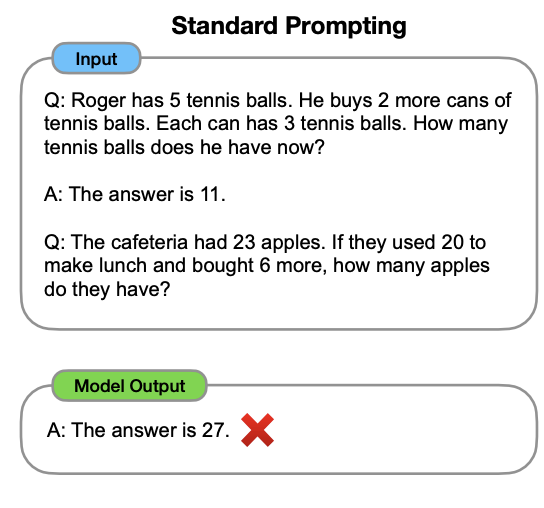
\includegraphics[height= 5in]{\images/ChainofThought1}}

\slide{Chain of Thought Prompting, January 2022}

\centerline{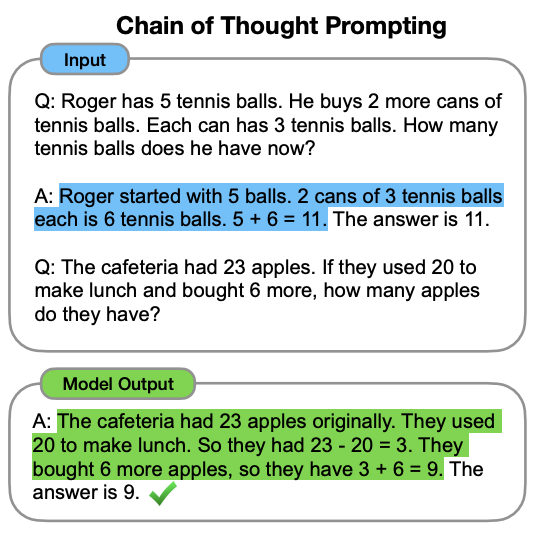
\includegraphics[height= 5in]{\images/ChainofThought2}}

\slide{Step by Step Prompting, June 2022}

It turns out that adding the simple instruction ``take it step by step'' elicits powerful chain of thought reasoning in GPT-3.

\slide{Humanoid Soccer, September 2022, Deep Mind}

Deep mind demonstrated two-on-two humanoid soccer in simulation (MuJoCo).

\vfill
This a startling advance in the state of the art in humanoid humanoid control.

\vfill
It also continues Deep Mind's effort in reinforcement learning.

\slide{Application Advancements vs. Architecture Advancements}

Advancements in the general principles of learning are having applications over very diverse applications.

\vfill
When considering Moore's law of AI it seems worth distinguishing architectural advancements (new general learning methods)
from new applications of established architectures.

\vfill
This course will focus on general, architectural, ideas.

\slideplain{END}

}
\end{document}
